
% Default to the notebook output style

    


% Inherit from the specified cell style.




    
\documentclass[11pt]{article}

    
    
    \usepackage[T1]{fontenc}
    % Nicer default font (+ math font) than Computer Modern for most use cases
    \usepackage{mathpazo}

    % Basic figure setup, for now with no caption control since it's done
    % automatically by Pandoc (which extracts ![](path) syntax from Markdown).
    \usepackage{graphicx}
    % We will generate all images so they have a width \maxwidth. This means
    % that they will get their normal width if they fit onto the page, but
    % are scaled down if they would overflow the margins.
    \makeatletter
    \def\maxwidth{\ifdim\Gin@nat@width>\linewidth\linewidth
    \else\Gin@nat@width\fi}
    \makeatother
    \let\Oldincludegraphics\includegraphics
    % Set max figure width to be 80% of text width, for now hardcoded.
    \renewcommand{\includegraphics}[1]{\Oldincludegraphics[width=.8\maxwidth]{#1}}
    % Ensure that by default, figures have no caption (until we provide a
    % proper Figure object with a Caption API and a way to capture that
    % in the conversion process - todo).
    \usepackage{caption}
    \DeclareCaptionLabelFormat{nolabel}{}
    \captionsetup{labelformat=nolabel}

    \usepackage{adjustbox} % Used to constrain images to a maximum size 
    \usepackage{xcolor} % Allow colors to be defined
    \usepackage{enumerate} % Needed for markdown enumerations to work
    \usepackage{geometry} % Used to adjust the document margins
    \usepackage{amsmath} % Equations
    \usepackage{amssymb} % Equations
    \usepackage{textcomp} % defines textquotesingle
    % Hack from http://tex.stackexchange.com/a/47451/13684:
    \AtBeginDocument{%
        \def\PYZsq{\textquotesingle}% Upright quotes in Pygmentized code
    }
    \usepackage{upquote} % Upright quotes for verbatim code
    \usepackage{eurosym} % defines \euro
    \usepackage[mathletters]{ucs} % Extended unicode (utf-8) support
    \usepackage[utf8x]{inputenc} % Allow utf-8 characters in the tex document
    \usepackage{fancyvrb} % verbatim replacement that allows latex
    \usepackage{grffile} % extends the file name processing of package graphics 
                         % to support a larger range 
    % The hyperref package gives us a pdf with properly built
    % internal navigation ('pdf bookmarks' for the table of contents,
    % internal cross-reference links, web links for URLs, etc.)
    \usepackage{hyperref}
    \usepackage{longtable} % longtable support required by pandoc >1.10
    \usepackage{booktabs}  % table support for pandoc > 1.12.2
    \usepackage[inline]{enumitem} % IRkernel/repr support (it uses the enumerate* environment)
    \usepackage[normalem]{ulem} % ulem is needed to support strikethroughs (\sout)
                                % normalem makes italics be italics, not underlines
    

    
    
    % Colors for the hyperref package
    \definecolor{urlcolor}{rgb}{0,.145,.698}
    \definecolor{linkcolor}{rgb}{.71,0.21,0.01}
    \definecolor{citecolor}{rgb}{.12,.54,.11}

    % ANSI colors
    \definecolor{ansi-black}{HTML}{3E424D}
    \definecolor{ansi-black-intense}{HTML}{282C36}
    \definecolor{ansi-red}{HTML}{E75C58}
    \definecolor{ansi-red-intense}{HTML}{B22B31}
    \definecolor{ansi-green}{HTML}{00A250}
    \definecolor{ansi-green-intense}{HTML}{007427}
    \definecolor{ansi-yellow}{HTML}{DDB62B}
    \definecolor{ansi-yellow-intense}{HTML}{B27D12}
    \definecolor{ansi-blue}{HTML}{208FFB}
    \definecolor{ansi-blue-intense}{HTML}{0065CA}
    \definecolor{ansi-magenta}{HTML}{D160C4}
    \definecolor{ansi-magenta-intense}{HTML}{A03196}
    \definecolor{ansi-cyan}{HTML}{60C6C8}
    \definecolor{ansi-cyan-intense}{HTML}{258F8F}
    \definecolor{ansi-white}{HTML}{C5C1B4}
    \definecolor{ansi-white-intense}{HTML}{A1A6B2}

    % commands and environments needed by pandoc snippets
    % extracted from the output of `pandoc -s`
    \providecommand{\tightlist}{%
      \setlength{\itemsep}{0pt}\setlength{\parskip}{0pt}}
    \DefineVerbatimEnvironment{Highlighting}{Verbatim}{commandchars=\\\{\}}
    % Add ',fontsize=\small' for more characters per line
    \newenvironment{Shaded}{}{}
    \newcommand{\KeywordTok}[1]{\textcolor[rgb]{0.00,0.44,0.13}{\textbf{{#1}}}}
    \newcommand{\DataTypeTok}[1]{\textcolor[rgb]{0.56,0.13,0.00}{{#1}}}
    \newcommand{\DecValTok}[1]{\textcolor[rgb]{0.25,0.63,0.44}{{#1}}}
    \newcommand{\BaseNTok}[1]{\textcolor[rgb]{0.25,0.63,0.44}{{#1}}}
    \newcommand{\FloatTok}[1]{\textcolor[rgb]{0.25,0.63,0.44}{{#1}}}
    \newcommand{\CharTok}[1]{\textcolor[rgb]{0.25,0.44,0.63}{{#1}}}
    \newcommand{\StringTok}[1]{\textcolor[rgb]{0.25,0.44,0.63}{{#1}}}
    \newcommand{\CommentTok}[1]{\textcolor[rgb]{0.38,0.63,0.69}{\textit{{#1}}}}
    \newcommand{\OtherTok}[1]{\textcolor[rgb]{0.00,0.44,0.13}{{#1}}}
    \newcommand{\AlertTok}[1]{\textcolor[rgb]{1.00,0.00,0.00}{\textbf{{#1}}}}
    \newcommand{\FunctionTok}[1]{\textcolor[rgb]{0.02,0.16,0.49}{{#1}}}
    \newcommand{\RegionMarkerTok}[1]{{#1}}
    \newcommand{\ErrorTok}[1]{\textcolor[rgb]{1.00,0.00,0.00}{\textbf{{#1}}}}
    \newcommand{\NormalTok}[1]{{#1}}
    
    % Additional commands for more recent versions of Pandoc
    \newcommand{\ConstantTok}[1]{\textcolor[rgb]{0.53,0.00,0.00}{{#1}}}
    \newcommand{\SpecialCharTok}[1]{\textcolor[rgb]{0.25,0.44,0.63}{{#1}}}
    \newcommand{\VerbatimStringTok}[1]{\textcolor[rgb]{0.25,0.44,0.63}{{#1}}}
    \newcommand{\SpecialStringTok}[1]{\textcolor[rgb]{0.73,0.40,0.53}{{#1}}}
    \newcommand{\ImportTok}[1]{{#1}}
    \newcommand{\DocumentationTok}[1]{\textcolor[rgb]{0.73,0.13,0.13}{\textit{{#1}}}}
    \newcommand{\AnnotationTok}[1]{\textcolor[rgb]{0.38,0.63,0.69}{\textbf{\textit{{#1}}}}}
    \newcommand{\CommentVarTok}[1]{\textcolor[rgb]{0.38,0.63,0.69}{\textbf{\textit{{#1}}}}}
    \newcommand{\VariableTok}[1]{\textcolor[rgb]{0.10,0.09,0.49}{{#1}}}
    \newcommand{\ControlFlowTok}[1]{\textcolor[rgb]{0.00,0.44,0.13}{\textbf{{#1}}}}
    \newcommand{\OperatorTok}[1]{\textcolor[rgb]{0.40,0.40,0.40}{{#1}}}
    \newcommand{\BuiltInTok}[1]{{#1}}
    \newcommand{\ExtensionTok}[1]{{#1}}
    \newcommand{\PreprocessorTok}[1]{\textcolor[rgb]{0.74,0.48,0.00}{{#1}}}
    \newcommand{\AttributeTok}[1]{\textcolor[rgb]{0.49,0.56,0.16}{{#1}}}
    \newcommand{\InformationTok}[1]{\textcolor[rgb]{0.38,0.63,0.69}{\textbf{\textit{{#1}}}}}
    \newcommand{\WarningTok}[1]{\textcolor[rgb]{0.38,0.63,0.69}{\textbf{\textit{{#1}}}}}
    
    
    % Define a nice break command that doesn't care if a line doesn't already
    % exist.
    \def\br{\hspace*{\fill} \\* }
    % Math Jax compatability definitions
    \def\gt{>}
    \def\lt{<}
    % Document parameters
    \title{tldr}
    
    
    

    % Pygments definitions
    
\makeatletter
\def\PY@reset{\let\PY@it=\relax \let\PY@bf=\relax%
    \let\PY@ul=\relax \let\PY@tc=\relax%
    \let\PY@bc=\relax \let\PY@ff=\relax}
\def\PY@tok#1{\csname PY@tok@#1\endcsname}
\def\PY@toks#1+{\ifx\relax#1\empty\else%
    \PY@tok{#1}\expandafter\PY@toks\fi}
\def\PY@do#1{\PY@bc{\PY@tc{\PY@ul{%
    \PY@it{\PY@bf{\PY@ff{#1}}}}}}}
\def\PY#1#2{\PY@reset\PY@toks#1+\relax+\PY@do{#2}}

\expandafter\def\csname PY@tok@w\endcsname{\def\PY@tc##1{\textcolor[rgb]{0.73,0.73,0.73}{##1}}}
\expandafter\def\csname PY@tok@c\endcsname{\let\PY@it=\textit\def\PY@tc##1{\textcolor[rgb]{0.25,0.50,0.50}{##1}}}
\expandafter\def\csname PY@tok@cp\endcsname{\def\PY@tc##1{\textcolor[rgb]{0.74,0.48,0.00}{##1}}}
\expandafter\def\csname PY@tok@k\endcsname{\let\PY@bf=\textbf\def\PY@tc##1{\textcolor[rgb]{0.00,0.50,0.00}{##1}}}
\expandafter\def\csname PY@tok@kp\endcsname{\def\PY@tc##1{\textcolor[rgb]{0.00,0.50,0.00}{##1}}}
\expandafter\def\csname PY@tok@kt\endcsname{\def\PY@tc##1{\textcolor[rgb]{0.69,0.00,0.25}{##1}}}
\expandafter\def\csname PY@tok@o\endcsname{\def\PY@tc##1{\textcolor[rgb]{0.40,0.40,0.40}{##1}}}
\expandafter\def\csname PY@tok@ow\endcsname{\let\PY@bf=\textbf\def\PY@tc##1{\textcolor[rgb]{0.67,0.13,1.00}{##1}}}
\expandafter\def\csname PY@tok@nb\endcsname{\def\PY@tc##1{\textcolor[rgb]{0.00,0.50,0.00}{##1}}}
\expandafter\def\csname PY@tok@nf\endcsname{\def\PY@tc##1{\textcolor[rgb]{0.00,0.00,1.00}{##1}}}
\expandafter\def\csname PY@tok@nc\endcsname{\let\PY@bf=\textbf\def\PY@tc##1{\textcolor[rgb]{0.00,0.00,1.00}{##1}}}
\expandafter\def\csname PY@tok@nn\endcsname{\let\PY@bf=\textbf\def\PY@tc##1{\textcolor[rgb]{0.00,0.00,1.00}{##1}}}
\expandafter\def\csname PY@tok@ne\endcsname{\let\PY@bf=\textbf\def\PY@tc##1{\textcolor[rgb]{0.82,0.25,0.23}{##1}}}
\expandafter\def\csname PY@tok@nv\endcsname{\def\PY@tc##1{\textcolor[rgb]{0.10,0.09,0.49}{##1}}}
\expandafter\def\csname PY@tok@no\endcsname{\def\PY@tc##1{\textcolor[rgb]{0.53,0.00,0.00}{##1}}}
\expandafter\def\csname PY@tok@nl\endcsname{\def\PY@tc##1{\textcolor[rgb]{0.63,0.63,0.00}{##1}}}
\expandafter\def\csname PY@tok@ni\endcsname{\let\PY@bf=\textbf\def\PY@tc##1{\textcolor[rgb]{0.60,0.60,0.60}{##1}}}
\expandafter\def\csname PY@tok@na\endcsname{\def\PY@tc##1{\textcolor[rgb]{0.49,0.56,0.16}{##1}}}
\expandafter\def\csname PY@tok@nt\endcsname{\let\PY@bf=\textbf\def\PY@tc##1{\textcolor[rgb]{0.00,0.50,0.00}{##1}}}
\expandafter\def\csname PY@tok@nd\endcsname{\def\PY@tc##1{\textcolor[rgb]{0.67,0.13,1.00}{##1}}}
\expandafter\def\csname PY@tok@s\endcsname{\def\PY@tc##1{\textcolor[rgb]{0.73,0.13,0.13}{##1}}}
\expandafter\def\csname PY@tok@sd\endcsname{\let\PY@it=\textit\def\PY@tc##1{\textcolor[rgb]{0.73,0.13,0.13}{##1}}}
\expandafter\def\csname PY@tok@si\endcsname{\let\PY@bf=\textbf\def\PY@tc##1{\textcolor[rgb]{0.73,0.40,0.53}{##1}}}
\expandafter\def\csname PY@tok@se\endcsname{\let\PY@bf=\textbf\def\PY@tc##1{\textcolor[rgb]{0.73,0.40,0.13}{##1}}}
\expandafter\def\csname PY@tok@sr\endcsname{\def\PY@tc##1{\textcolor[rgb]{0.73,0.40,0.53}{##1}}}
\expandafter\def\csname PY@tok@ss\endcsname{\def\PY@tc##1{\textcolor[rgb]{0.10,0.09,0.49}{##1}}}
\expandafter\def\csname PY@tok@sx\endcsname{\def\PY@tc##1{\textcolor[rgb]{0.00,0.50,0.00}{##1}}}
\expandafter\def\csname PY@tok@m\endcsname{\def\PY@tc##1{\textcolor[rgb]{0.40,0.40,0.40}{##1}}}
\expandafter\def\csname PY@tok@gh\endcsname{\let\PY@bf=\textbf\def\PY@tc##1{\textcolor[rgb]{0.00,0.00,0.50}{##1}}}
\expandafter\def\csname PY@tok@gu\endcsname{\let\PY@bf=\textbf\def\PY@tc##1{\textcolor[rgb]{0.50,0.00,0.50}{##1}}}
\expandafter\def\csname PY@tok@gd\endcsname{\def\PY@tc##1{\textcolor[rgb]{0.63,0.00,0.00}{##1}}}
\expandafter\def\csname PY@tok@gi\endcsname{\def\PY@tc##1{\textcolor[rgb]{0.00,0.63,0.00}{##1}}}
\expandafter\def\csname PY@tok@gr\endcsname{\def\PY@tc##1{\textcolor[rgb]{1.00,0.00,0.00}{##1}}}
\expandafter\def\csname PY@tok@ge\endcsname{\let\PY@it=\textit}
\expandafter\def\csname PY@tok@gs\endcsname{\let\PY@bf=\textbf}
\expandafter\def\csname PY@tok@gp\endcsname{\let\PY@bf=\textbf\def\PY@tc##1{\textcolor[rgb]{0.00,0.00,0.50}{##1}}}
\expandafter\def\csname PY@tok@go\endcsname{\def\PY@tc##1{\textcolor[rgb]{0.53,0.53,0.53}{##1}}}
\expandafter\def\csname PY@tok@gt\endcsname{\def\PY@tc##1{\textcolor[rgb]{0.00,0.27,0.87}{##1}}}
\expandafter\def\csname PY@tok@err\endcsname{\def\PY@bc##1{\setlength{\fboxsep}{0pt}\fcolorbox[rgb]{1.00,0.00,0.00}{1,1,1}{\strut ##1}}}
\expandafter\def\csname PY@tok@kc\endcsname{\let\PY@bf=\textbf\def\PY@tc##1{\textcolor[rgb]{0.00,0.50,0.00}{##1}}}
\expandafter\def\csname PY@tok@kd\endcsname{\let\PY@bf=\textbf\def\PY@tc##1{\textcolor[rgb]{0.00,0.50,0.00}{##1}}}
\expandafter\def\csname PY@tok@kn\endcsname{\let\PY@bf=\textbf\def\PY@tc##1{\textcolor[rgb]{0.00,0.50,0.00}{##1}}}
\expandafter\def\csname PY@tok@kr\endcsname{\let\PY@bf=\textbf\def\PY@tc##1{\textcolor[rgb]{0.00,0.50,0.00}{##1}}}
\expandafter\def\csname PY@tok@bp\endcsname{\def\PY@tc##1{\textcolor[rgb]{0.00,0.50,0.00}{##1}}}
\expandafter\def\csname PY@tok@fm\endcsname{\def\PY@tc##1{\textcolor[rgb]{0.00,0.00,1.00}{##1}}}
\expandafter\def\csname PY@tok@vc\endcsname{\def\PY@tc##1{\textcolor[rgb]{0.10,0.09,0.49}{##1}}}
\expandafter\def\csname PY@tok@vg\endcsname{\def\PY@tc##1{\textcolor[rgb]{0.10,0.09,0.49}{##1}}}
\expandafter\def\csname PY@tok@vi\endcsname{\def\PY@tc##1{\textcolor[rgb]{0.10,0.09,0.49}{##1}}}
\expandafter\def\csname PY@tok@vm\endcsname{\def\PY@tc##1{\textcolor[rgb]{0.10,0.09,0.49}{##1}}}
\expandafter\def\csname PY@tok@sa\endcsname{\def\PY@tc##1{\textcolor[rgb]{0.73,0.13,0.13}{##1}}}
\expandafter\def\csname PY@tok@sb\endcsname{\def\PY@tc##1{\textcolor[rgb]{0.73,0.13,0.13}{##1}}}
\expandafter\def\csname PY@tok@sc\endcsname{\def\PY@tc##1{\textcolor[rgb]{0.73,0.13,0.13}{##1}}}
\expandafter\def\csname PY@tok@dl\endcsname{\def\PY@tc##1{\textcolor[rgb]{0.73,0.13,0.13}{##1}}}
\expandafter\def\csname PY@tok@s2\endcsname{\def\PY@tc##1{\textcolor[rgb]{0.73,0.13,0.13}{##1}}}
\expandafter\def\csname PY@tok@sh\endcsname{\def\PY@tc##1{\textcolor[rgb]{0.73,0.13,0.13}{##1}}}
\expandafter\def\csname PY@tok@s1\endcsname{\def\PY@tc##1{\textcolor[rgb]{0.73,0.13,0.13}{##1}}}
\expandafter\def\csname PY@tok@mb\endcsname{\def\PY@tc##1{\textcolor[rgb]{0.40,0.40,0.40}{##1}}}
\expandafter\def\csname PY@tok@mf\endcsname{\def\PY@tc##1{\textcolor[rgb]{0.40,0.40,0.40}{##1}}}
\expandafter\def\csname PY@tok@mh\endcsname{\def\PY@tc##1{\textcolor[rgb]{0.40,0.40,0.40}{##1}}}
\expandafter\def\csname PY@tok@mi\endcsname{\def\PY@tc##1{\textcolor[rgb]{0.40,0.40,0.40}{##1}}}
\expandafter\def\csname PY@tok@il\endcsname{\def\PY@tc##1{\textcolor[rgb]{0.40,0.40,0.40}{##1}}}
\expandafter\def\csname PY@tok@mo\endcsname{\def\PY@tc##1{\textcolor[rgb]{0.40,0.40,0.40}{##1}}}
\expandafter\def\csname PY@tok@ch\endcsname{\let\PY@it=\textit\def\PY@tc##1{\textcolor[rgb]{0.25,0.50,0.50}{##1}}}
\expandafter\def\csname PY@tok@cm\endcsname{\let\PY@it=\textit\def\PY@tc##1{\textcolor[rgb]{0.25,0.50,0.50}{##1}}}
\expandafter\def\csname PY@tok@cpf\endcsname{\let\PY@it=\textit\def\PY@tc##1{\textcolor[rgb]{0.25,0.50,0.50}{##1}}}
\expandafter\def\csname PY@tok@c1\endcsname{\let\PY@it=\textit\def\PY@tc##1{\textcolor[rgb]{0.25,0.50,0.50}{##1}}}
\expandafter\def\csname PY@tok@cs\endcsname{\let\PY@it=\textit\def\PY@tc##1{\textcolor[rgb]{0.25,0.50,0.50}{##1}}}

\def\PYZbs{\char`\\}
\def\PYZus{\char`\_}
\def\PYZob{\char`\{}
\def\PYZcb{\char`\}}
\def\PYZca{\char`\^}
\def\PYZam{\char`\&}
\def\PYZlt{\char`\<}
\def\PYZgt{\char`\>}
\def\PYZsh{\char`\#}
\def\PYZpc{\char`\%}
\def\PYZdl{\char`\$}
\def\PYZhy{\char`\-}
\def\PYZsq{\char`\'}
\def\PYZdq{\char`\"}
\def\PYZti{\char`\~}
% for compatibility with earlier versions
\def\PYZat{@}
\def\PYZlb{[}
\def\PYZrb{]}
\makeatother


    % Exact colors from NB
    \definecolor{incolor}{rgb}{0.0, 0.0, 0.5}
    \definecolor{outcolor}{rgb}{0.545, 0.0, 0.0}



    
    % Prevent overflowing lines due to hard-to-break entities
    \sloppy 
    % Setup hyperref package
    \hypersetup{
      breaklinks=true,  % so long urls are correctly broken across lines
      colorlinks=true,
      urlcolor=urlcolor,
      linkcolor=linkcolor,
      citecolor=citecolor,
      }
    % Slightly bigger margins than the latex defaults
    
    \geometry{verbose,tmargin=1in,bmargin=1in,lmargin=1in,rmargin=1in}
    
    

    \begin{document}
    
    
    \maketitle
    
    

    
    \section{tl;dr}\label{tldr}

\subsubsection{A text summarizer}\label{a-text-summarizer}

\subsubsection{Sanjay Dorairaj}\label{sanjay-dorairaj}

    \section{Abstract}\label{abstract}

The title of this paper is tl;dr (too long don't read). The goal of this
work is to create a neural network based multi-line text summarizer
building on state of the art methods that exist today. The final goal of
this work is to incorporate this summarizer into various applications in
need of this feature, such as, websites (via a Chrome, Firefox plugin or
similar) and in blog sites and wikis.

The internet and other catalysts such as big data have set the stage for
the exponential growth of available information. This information often
manifests itself in news articles, blogs, research papers, social media
conversations and so on. Consuming and keeping track of all this
information is extremely difficult. While on the one hand, information
provides a definite edge and opens doors to new opportunities,
navigating and keeping track of the flood of information is impossible
since our single-processor minds lack the capacity to process all this
information.

The parallel processing capability of computers (read GPUs) and the
advances in neural network technologies however, can help us get closer
to our goal of fishing meaningful information i.e. information that
matters to us, from the vast ocean of available information.

For a long time, the primary method of delivering meaningful information
to users has been through information retrieval and recommendation
models. Take for example, Google's Page Rank algorithm {[}1{]}. This
algorithm ranks all pages on the internet in order of quality based on
how many sites recommend (or point to) a site. Other recommendation
models perform custom recommendations, where information content is
matched based on other users with similar tastes or similar articles
consumed in the past. While these approaches help reduce the amount of
information directed at its consumer, the filtered information is itself
sufficiently large for any one individual to process. Text summarizers
attempt to deal with this second issue. By compressing text into
byte-sized pieces, they help minimize consumption time bringing us even
closer to our goal of being "up to date".

This paper examines some of the latest advances in text summarization
and attempts to build upon past work to create a relatively more
effective text summarizer. The keys ideas explored in this paper are the
RNN/LSTM based sequence-to-sequence network, attention,
pointer-generation, beam search and the noisy channel model.

\textless{}\textless{} FINDINGS \textgreater{}\textgreater{}

\textbf{Note}

All diagrams are not final and will be updated later to be more
professional grade :-)

    \section{Introduction}\label{introduction}

Here, we introduce various techniques of text summarization that are
available today and key definitions and nomenclature surrounding these
techniques. We also talk about the key ideas used in this paper and how
these ideas differ from existing research.

There are two popular forms of text summarization - extractive and
abstractive {[}2{]} . Extractive text summmarization seeks to reproduce
parts of the input text in the output text summary. On the other hand,
abstractive text summarization takes a more creative approach. It
attempts to summarize by creating an original sequence of words that
attempt to capture the gist of the input text. This method has been
traditionally difficult to implement since it requires a fundamental
understanding of creative sentence construction which has eluded us for
a long time. However, with the recent advances in neural networks,
especially in the area of recursive neural networks or RNNs, we appear
to be closer to our goal of creative sentence construction.

Although a vanilla sequence to sequence (or encoder/decoder) networks
give us a good start they have the following issues (1) they
inaccurately reproduce factual details, (2) have issues dealing with out
of vocabulary words (OOV) and 3) repeat themselves (sic {[}2{]}). The
beam search algorithm is used to help pick the best complete output
sentence by conditioning each decoder output on previously emitted
words. Attention models {[}3{]} help deal with the first issue, while
pointer generation models help deal with the second issue. {[}2{]}
suggests using a coverage model to deal with the issue of repeating
words. In this paper we take a slightly different approach. The last
beam search decision or prioritization is conditioned upon the
probability of the output being grammatically correct. The POS validator
is an independently generated classifer model.

This paper pulls together the latest ideas in sequence to sequence
networks, attention, beam search and pointer-generation networks. It
enhances this framework with a parts of speech based (POS) noisy channel
model for optimizing beam search performance.

    \section{Background}\label{background}

In this section we explain each of the technologies that are used in
this paper.

\subsection{Sequence to sequence
models}\label{sequence-to-sequence-models}

A sequence to sequence network {[}4{]} is also referred to an
encoder-decoder model. This model allows us to generate a sequence of
output corresponding to a given input sequence. The model typically uses
an enhanced RNN cell, such as a bi-LSTM, multi-stacked model, in order
to process input text. The bi-LSTM allows the model to leverage both the
future and the past to make predictions and the LSTMs address the issue
of vanishing or exploding gradients. This part of the processing happens
in the encoder network. The last hidden state of the encoder network is
expected to hold knowledge of the entire input sentence. This is fed
into another LSTM network, known as the decoder network. The decoder
network takes as input the last hidden state from the encoder network
and the previous output word and generates the next word. The decoder
stops generating words when it generates a special word that denotes the
end of the output sequence.

\begin{figure}
\centering
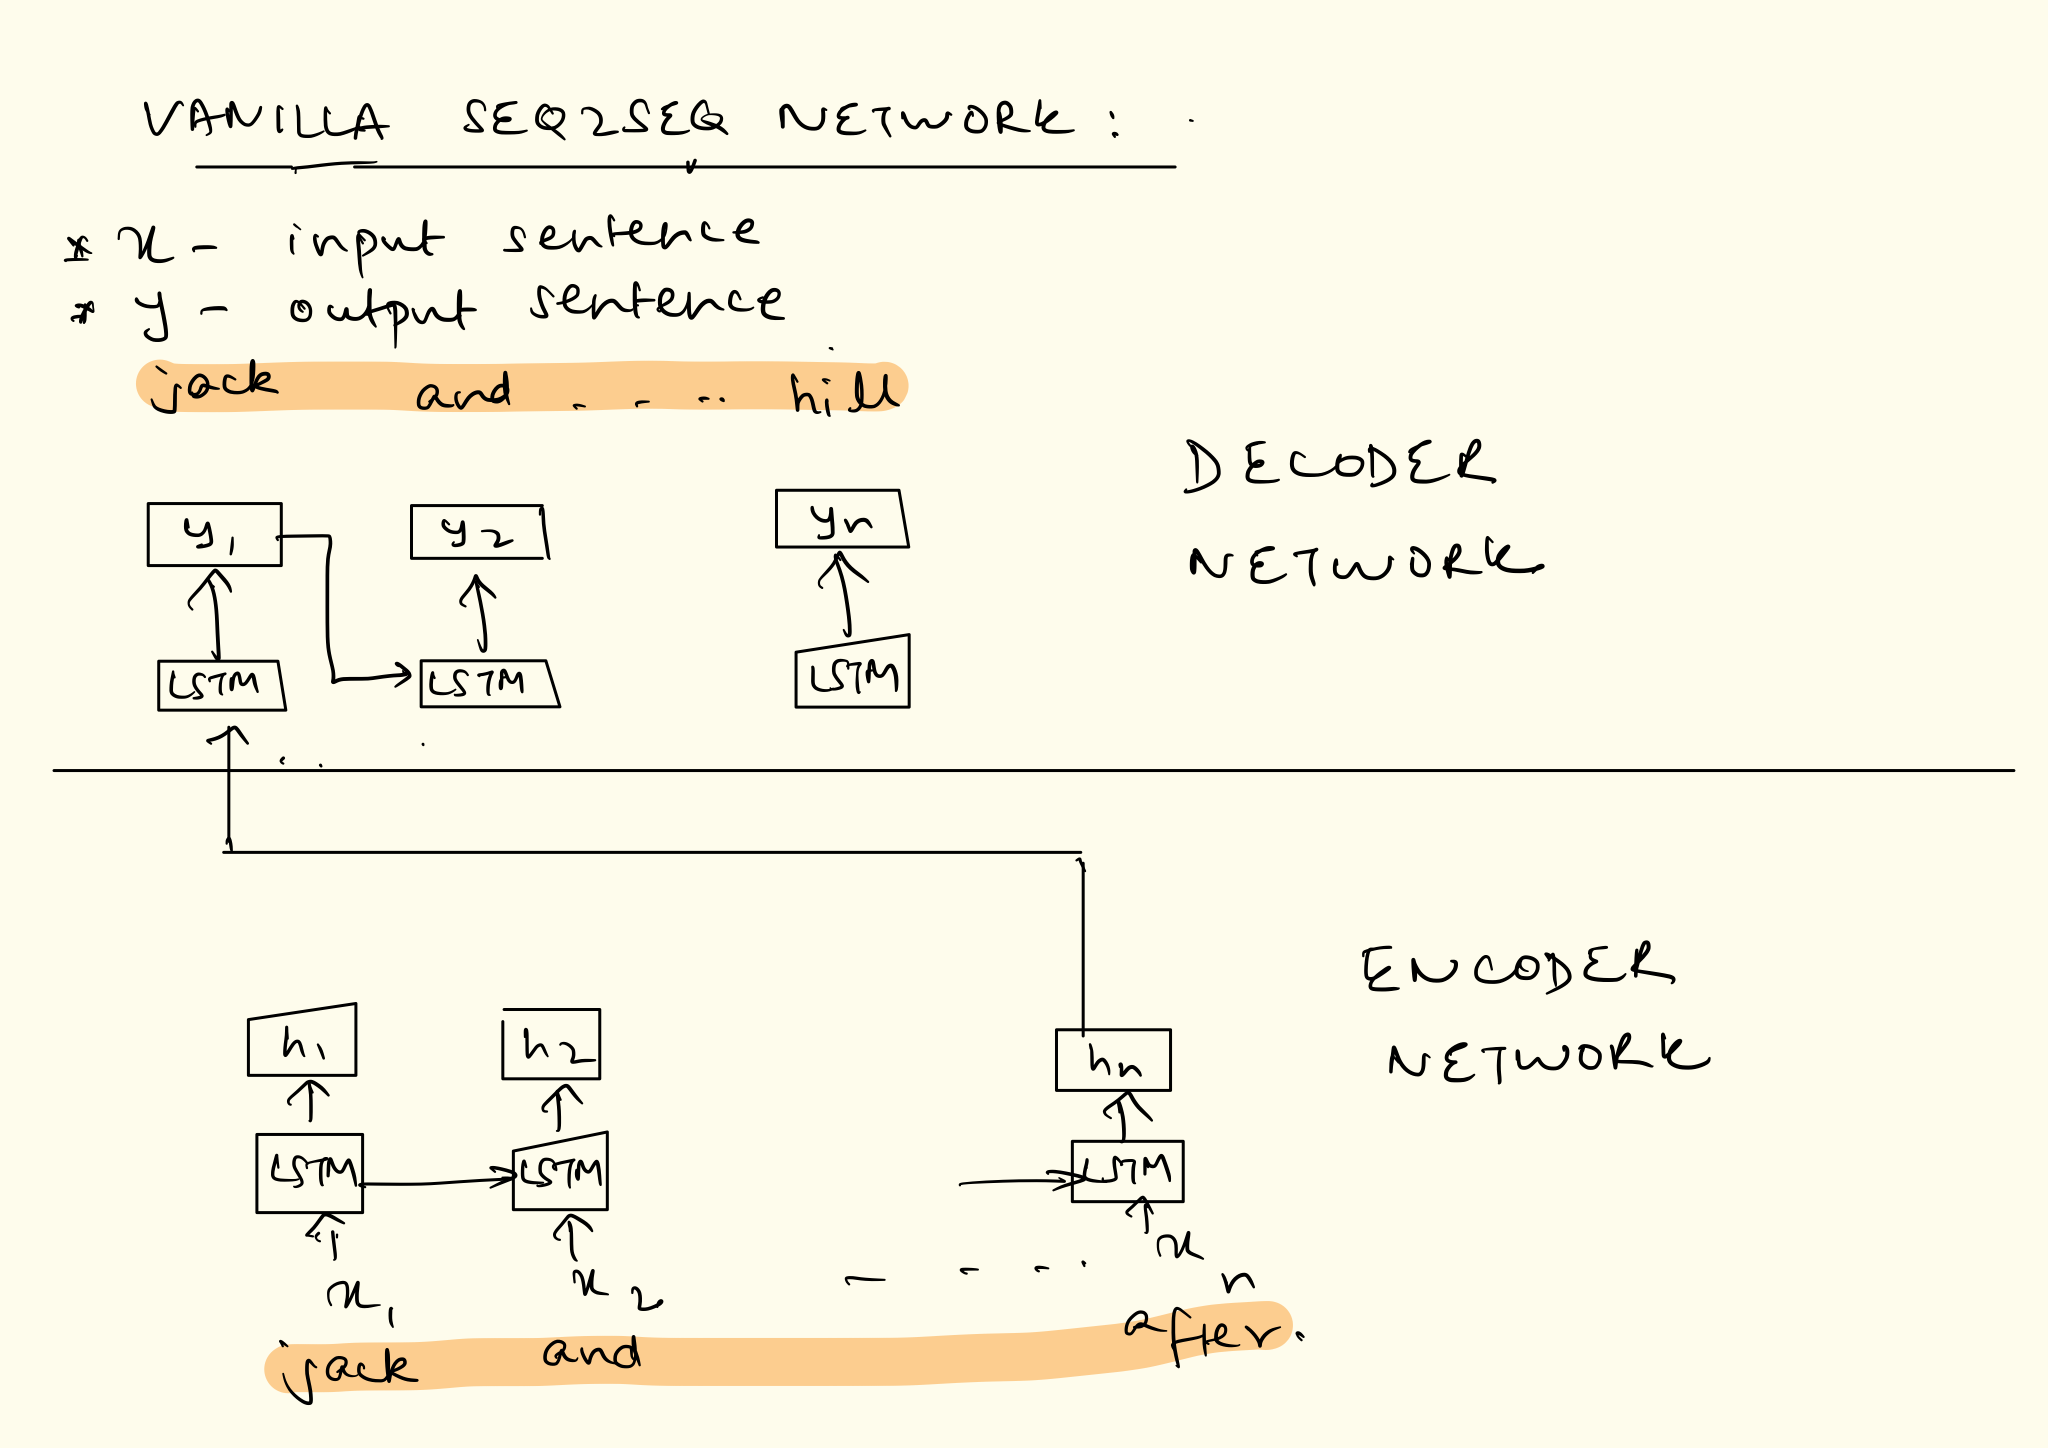
\includegraphics{vanilla-seq2seq-network.png}
\caption{Seq2seq Network}
\end{figure}

 ** Figure 1: Vanilla Sequence to Sequence Network **

Key considerations when designing a sequence to sequence network during
text summarization is to ensure that each summary is to ensure that
during training each summary is terminated with a special end of
sequence of token. During inference, we stop sentence generation when we
see this end of sequence token. Also, we use a dual-stacked
bidirectional LSTM for our base model.

    \subsection{Attention models}\label{attention-models}

The problem with vanilla sequence to sequence networks in the contex of
text summarization is that they have been shown to generate inaccurate
details of the undelying input text {[}2{]}. The reason for this has
been largely attributed to the model's inability to compress all
information about the piece of input text into a single hidden vector
i.e. even LSTMs tend to forget critical information if they need to
process large amount of text.

Attention-based models attempt to fix this issue by allowing the decoder
to glimpse the details of encoder processing and factor this information
into output generation. This is analogous to how humans summarize
information when looking at large volumes of text. Rather than trying to
read the entire text and summarizing, we summarize a block of text and
move on to summarizing the next contiguous block and so on.
Attention-based models attempt to keep the decoder informed of the
relative priority of words in the input text, so that the decoder can
focus on relevant parts of the input text during the summarization
process.

\begin{figure}
\centering
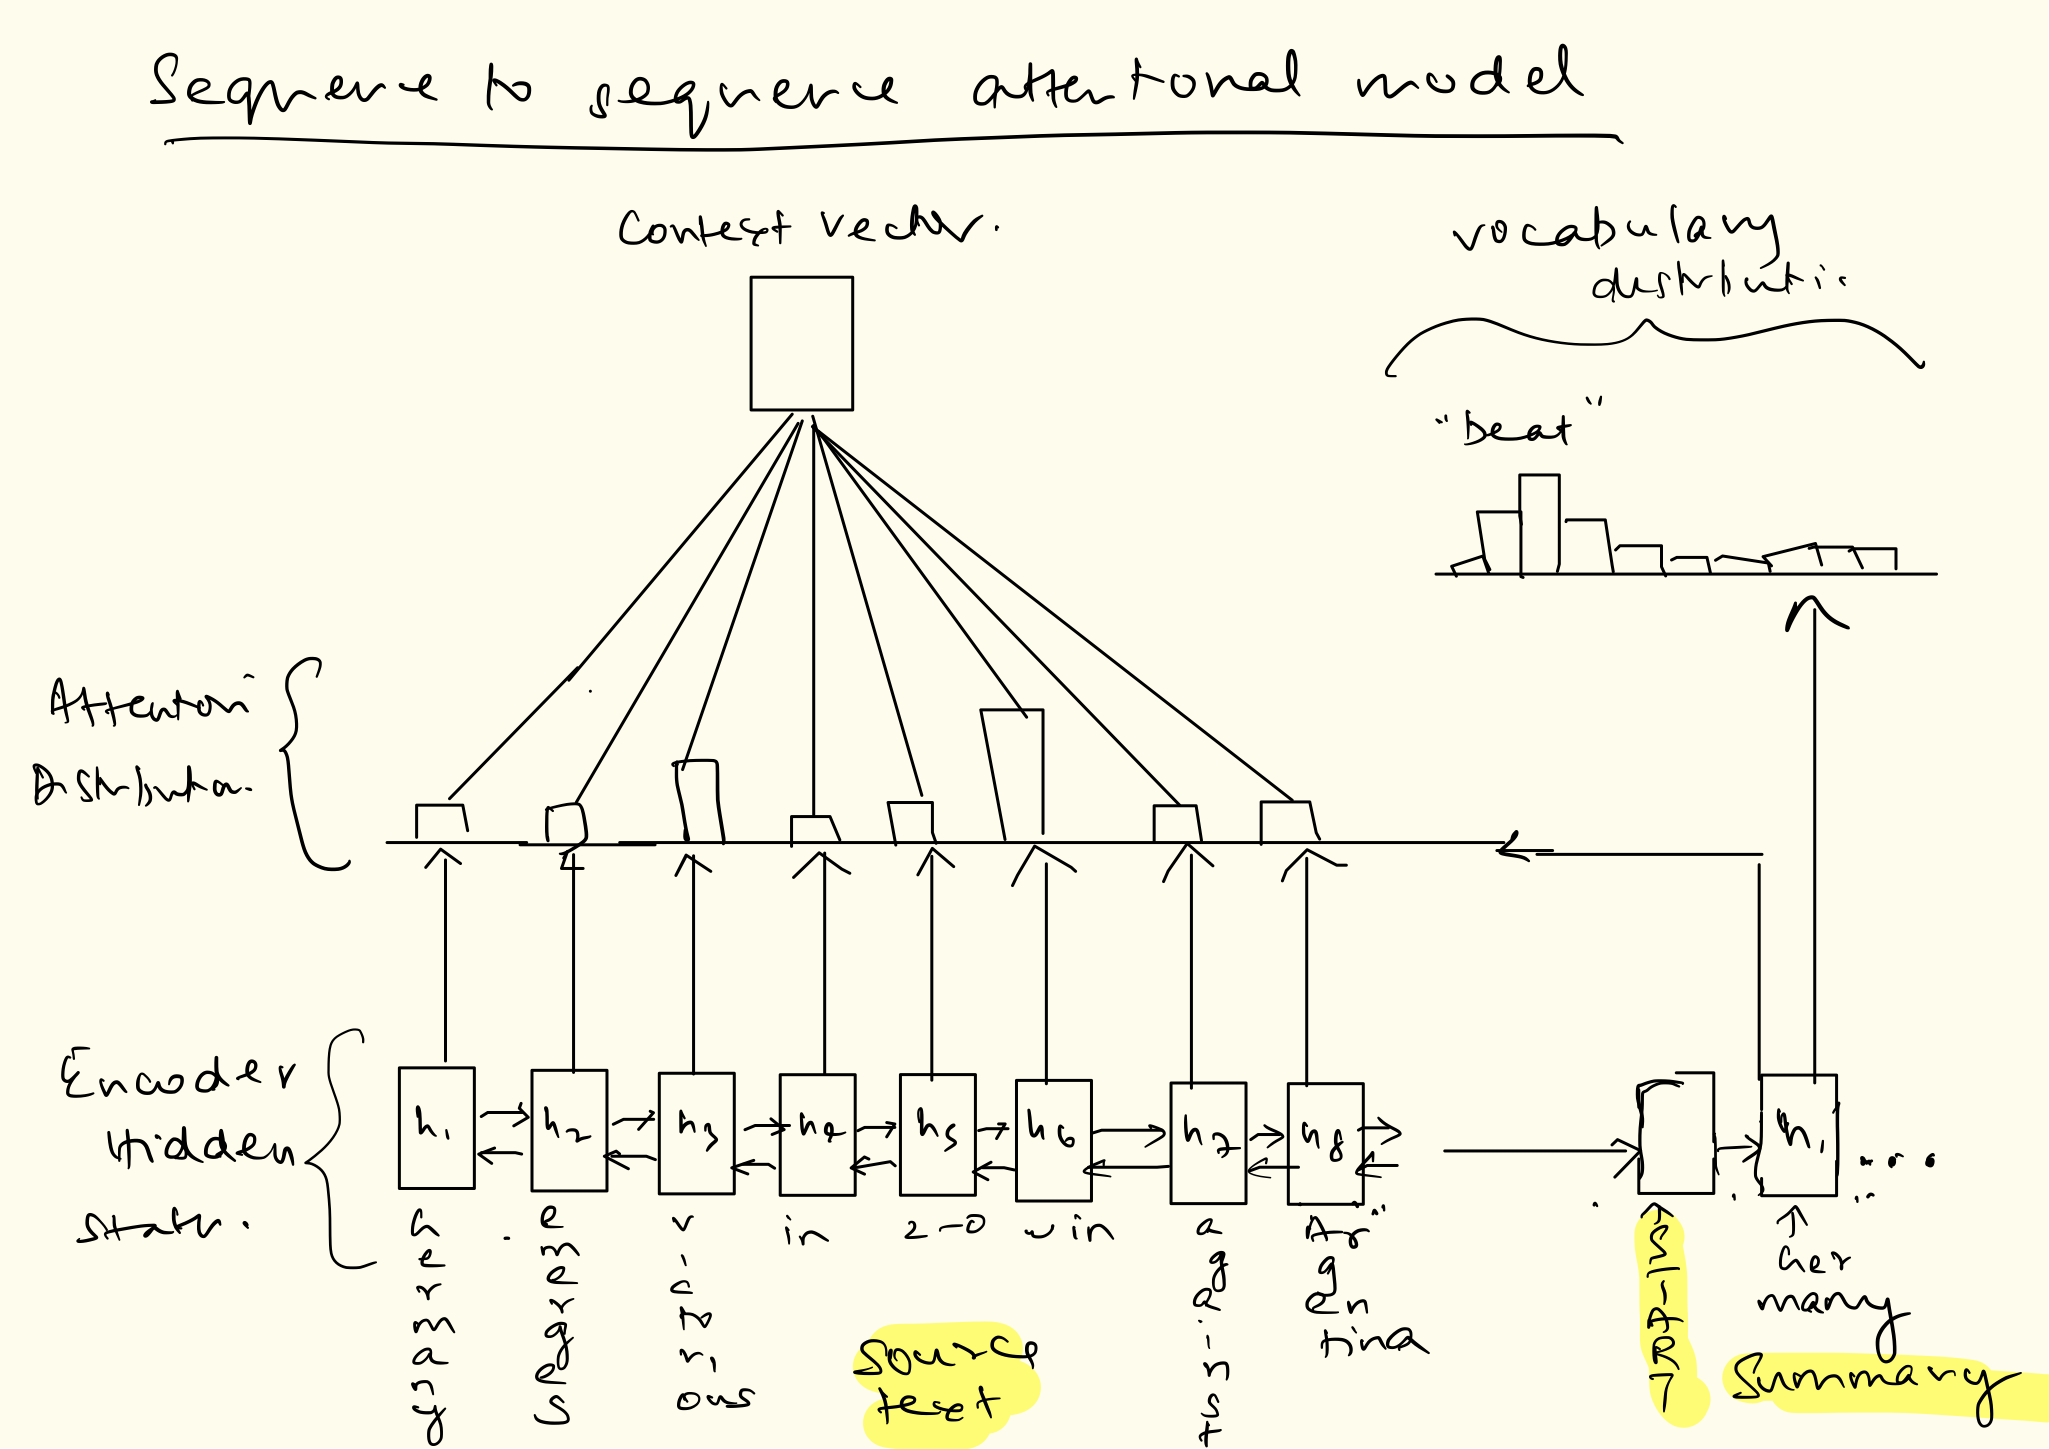
\includegraphics{seq2seq-attn.png}
\caption{Seq2Seq Network with Attention}
\end{figure}

 ** Figure 2: Sequence to Sequence Network with Attention ** Source: Get
To the Point: Summarization with Pointer-Generator {[}2{]} 

    The actual implementation of attention is relatively straightforward.
The process of using attention is depicted realy well in the picture
below extracted from Chris Dyer's slides on Modeling with Attention. For
each forward and backward pass of a bi-directional LSTM, hidden state
information is concatenated to create a column in an MXN matrix F, where
M is the size of the hidden dimension and N is the number of words in
the input sentence. A weight matrix, V, is then learned to compute an
expected input embedding \$r\_t for each previous decoder input
\(s_{t-1}\).

\(r_{t} = Vs_{t-1}\)

An attention vector for each decoder state \$s\{t-1\} using the equation
below

\(e_t = F^Tr_{t}\),

\(e_t\) is known as the attention energy. It is exponentiated and
normalized and then multipled with our matrix F, in order to yield a
context vector \(C_{t}\)

This context vector is fed along with \(s_{t-1}\) as input into the next
step of the decoder allowing the decoder to catch glimpses of the
encoder hidden states and use this information to inform the decoding
process.

 ** Figure 3: Inferring Attention in a Sequence to Sequence Network **
Source: Lecture 8 - Generation Language with Attention, Chris Dyer
{[}5{]}

    \subsection{Pointer Generation}\label{pointer-generation}

A Pointer generation model allows for the model to handle out of
vocabulary (OOV) words. At each timestep, the model chooses between
whether to use abstractive output from the decoder or whether to pull
information from the pointer generation mechanism. More details about
this approach can be found in {[}2{]}

    \subsection{Beam Search with Noisy Channel
model}\label{beam-search-with-noisy-channel-model}

The Beam Search algorithm allows us to generate output text that has a
higher likelihood of occuring given the input text. It does this by
conditioning output words during each step of the decoding process on
the input text and picking partial text that has a higher likelihood of
occuring for a given input sentence. Beam search tries different
combinations of partial output sentences, each time picking a set of
partial output sentences with the highest likelihood. The process
repeats until we generate the full sentence. At this point, we repeat
our conditional probability computation one last time and pick the
winning sentence.

The picture below provides a nice overview of the beam search algorithm.

 ** Figure 4: Overview of Beam Search ** Source:
https://github.com/mfederico and
https://www.quora.com/Why-is-beam-search-required-in-sequence-to-sequence-transduction-using-recurrent-neural-networks

    \subsubsection{POS based Noisy Channel
model}\label{pos-based-noisy-channel-model}

The POS-based noisy channel model is provided as an augmentation to the
beam search algorithm and is applied during the last phase of beam
search when all possible full sentence outputs are known. A
POS-validation is performed on each of the sentences in rank order of
conditional likelihood. The first sentence that passes POS validation is
selected as the final output sentence.

This is shown in the diagram below

 ** Figure 5: Parts of Speech Vaidation on Beam Search output **

The POS validation model is a binary classifier that is trained on valid
and invalid parts of speech tags using negative sampling techniques.

    \subsection{Validation metrics - ROUGE
score}\label{validation-metrics---rouge-score}

The ROUGE score is a standad method for evaluation of text
summarization. We will use this same metric in order to validate out
text summarization as well.

ROUGE stands for Recall-Oriented Understudy for Gisting Evaluation
{[}7{]}. It comapres an automatically produced summary against a set of
reference summaries. In the context of the ROUGE score, a higher recall
corresponds to recalling more words from the reference summaries.
Precision looks at the number of overlapping words relative to the total
words output by the system. Thus precision decreases as the number of
spurious words in the system generated output summary decreases.

The ROUGE score is compared on n-grams - typically unigrams and bigrams.

Another version of the ROUGE score, called ROUGE-S measures the longest
matching sequence of words.

We will be using one of several available packages for evaluating the
ROUGE score of our output summaries.

    \section{Methods}\label{methods}

This section captures various implementation details of this paper.

There are several similarities between this paper and other existing
state of the art papers on text summarization.

\begin{enumerate}
\def\labelenumi{\arabic{enumi}.}
\tightlist
\item
  Use of sequence to sequence models.
\item
  Use of attention-based models
\item
  Use of pointer-generation networks
\item
  Use of beam search to select the best output sequence
\item
  Use of CNN/Daily Mail dataset.
\item
  Use of pre-trained Glove embeddings to encode input sentences.
\end{enumerate}

The primary areas where this paper differs from the above papers are
listed below

\begin{enumerate}
\def\labelenumi{\arabic{enumi}.}
\tightlist
\item
  Use of a POS-based validator in the final phase of Beam search.
\item
  Hyperparameter tuning to ensure best results.
\end{enumerate}

\subsection{Model}\label{model}

In this section, we outline the various steps in the construction of
this model.

The steps involved in the model are as follows

\begin{enumerate}
\def\labelenumi{\arabic{enumi}.}
\tightlist
\item
  Input text is first converted into word embeddings using pretrained
  Glove embeddings.
\item
  This is fed into a decoder, a bi-directional LSTM network.
\item
  The output of the encoder is fed into the decoder LSTM network, a
  unidirectional LSTM.
\item
  Attention weights are computed from the hidden weights and output
  states for each timestep.
\item
  A pointer generation model weights are computed to determine whether
  the next word should be selected from the decoder or directly from the
  output text.\\
\item
  Decoder output goes through a beam search at each timestep to get a
  set of k possible best matches, where k is the beam size.
\item
  In the final step of the decoder, a Parts of Speech (POS) classifer is
  used to select the first highest rank beam search output that passes
  POS validation.
\end{enumerate}

These steps are captured in the block diagram below.

 ** Figure 6: End to End Block Diagram of Text Summarizer **

\subsubsection{Preliminary model
parameters}\label{preliminary-model-parameters}

The following are initial parameters to the model. Final hyperparameters
will be determined following hyper-parameters which takes place during
the actual experimentation phase.

\begin{enumerate}
\def\labelenumi{\arabic{enumi}.}
\tightlist
\item
  Encoder - Bidirectional LSTM
\item
  Decoder - Unidirectional LSTM
\item
  Hidden Dimension - 500
\item
  Embedding Dimension - 500
\item
  Beam size for beam search - 3
\item
  Hardware/Software resources - Google Cloud Platform.
\end{enumerate}

    \subsection{Experimentation}\label{experimentation}

This section captures the experimentation and data collection steps.

    \subsubsection{Baseline Sequence to Sequence
Model}\label{baseline-sequence-to-sequence-model}

In this section, we build a baseline model for text summarization using
a vanialla sequence to sequence network. This is similar to the network
shown in Figure 1 above.

    \begin{Verbatim}[commandchars=\\\{\}]
{\color{incolor}In [{\color{incolor}1}]:} \PY{c+c1}{\PYZsh{}\PYZsh{}\PYZsh{}\PYZsh{} Loading CNN dataset}
        
        \PY{k+kn}{import} \PY{n+nn}{pickle}
        
        \PY{n}{stories} \PY{o}{=} \PY{n}{pickle}\PY{o}{.}\PY{n}{load}\PY{p}{(}\PY{n+nb}{open}\PY{p}{(}\PY{l+s+s1}{\PYZsq{}}\PY{l+s+s1}{cnn\PYZus{}dataset.pkl}\PY{l+s+s1}{\PYZsq{}}\PY{p}{,} \PY{l+s+s1}{\PYZsq{}}\PY{l+s+s1}{rb}\PY{l+s+s1}{\PYZsq{}}\PY{p}{)}\PY{p}{)}
        \PY{n+nb}{print}\PY{p}{(}\PY{l+s+s1}{\PYZsq{}}\PY{l+s+s1}{Loaded Stories }\PY{l+s+si}{\PYZpc{}d}\PY{l+s+s1}{\PYZsq{}} \PY{o}{\PYZpc{}} \PY{n+nb}{len}\PY{p}{(}\PY{n}{stories}\PY{p}{)}\PY{p}{)}
\end{Verbatim}


    \begin{Verbatim}[commandchars=\\\{\}]
Loaded Stories 92579

    \end{Verbatim}

    \begin{Verbatim}[commandchars=\\\{\}]
{\color{incolor}In [{\color{incolor}2}]:} \PY{c+c1}{\PYZsh{}\PYZsh{}\PYZsh{} Generate a sequence to sequence baseline model.}
        
        \PY{c+c1}{\PYZsh{} \PYZlt{}tbd\PYZgt{}}
\end{Verbatim}


    \subsubsection{Dataset}\label{dataset}

The dataset for this model is the CNN/Dailymail dataset{[}6{]}. The
reason we choose this dataset over other datasets is because this has
larger abstracts, whereas most other datasets have single sentence
summaries (or headlines). We are interested in generating summaries that
span multiple sentences (recall our earlier goal of generating multiline
text summaries).

The data is split into 70:30 for \textbf{training} and
\textbf{validation}. Training involves k-fold cross-verification to
allow for hyperparameter tuning.

\subsubsection{Training}\label{training}

TBD

\subsubsection{Validation}\label{validation}

TBD

    \section{Results and discussion}\label{results-and-discussion}

TBD

    \section{Next Steps}\label{next-steps}

TBD

    \section{References}\label{references}

    \begin{enumerate}
\def\labelenumi{\arabic{enumi}.}
\tightlist
\item
  The Anatomy of a Large-Scale Hypertextual Web Search Engine,
  http://infolab.stanford.edu/\textasciitilde{}backrub/google.html
\item
  Get to the Point: Summarization with Pointer-Generator Networks,
  https://arxiv.org/abs/1704.04368
\item
  Neural Machine Translation by Jointly Learning to Align and Translate,
  https://arxiv.org/abs/1409.0473
\item
  Sequence to Sequence Learning with Neural Networks,
  https://papers.nips.cc/paper/5346-sequence-to-sequence-learning-with-neural-networks.pdf
\item
  Modeling with Attention, Lecture 8, Chris Dyer, CMU,
  https://www.youtube.com/watch?v=ah7\_mfl7LD0\&t=241s
\item
  CNN/Dailymail dataset, https://cs.nyu.edu/\textasciitilde{}kcho/DMQA/
\item
  What is ROUGE and How it works for Evaluation of Summarization Tasks?,
  http://rxnlp.com/how-rouge-works-for-evaluation-of-summarization-tasks/\#.WrmhF9PwZTY
\end{enumerate}


    % Add a bibliography block to the postdoc
    
    
    
    \end{document}
